
% This LaTeX was auto-generated from MATLAB code.
% To make changes, update the MATLAB code and republish this document.

\documentclass{article}
\usepackage{graphicx}
\usepackage{color}

\sloppy
\definecolor{lightgray}{gray}{0.5}
\setlength{\parindent}{0pt}

\begin{document}

    
    \begin{verbatim}
function fourthTask
t0=0;
t0=fsolve(@function1,t0);
x0=[-0.3,t0];
[t,x]=ode45(@function2,[1,4],x0);
figure(4),plot(t,x(:,1),t,x(:,2),'r')
xlabel('t');
ylabel('x(t)');
legend('x(t)', "x'(t)", 'Location', 'northeast');
title('Решение по метода на стрелбата');
end

function f=function1(x)
x0=[-0.3,x];
[t,x]=ode45(@function2,[1,4],x0);
n=length(t);
f=x(n,1)-0.4;
end

function dy=function2(t,x)
dy(1,1)=x(2);
dy(2,1)=sin(1/t^2)-(16/t^2)-(x(1)/t);
end
\end{verbatim}

        \color{lightgray} \begin{verbatim}
Equation solved.

fsolve completed because the vector of function values is near zero
as measured by the value of the function tolerance, and
the problem appears regular as measured by the gradient.

\end{verbatim} \color{black}
    
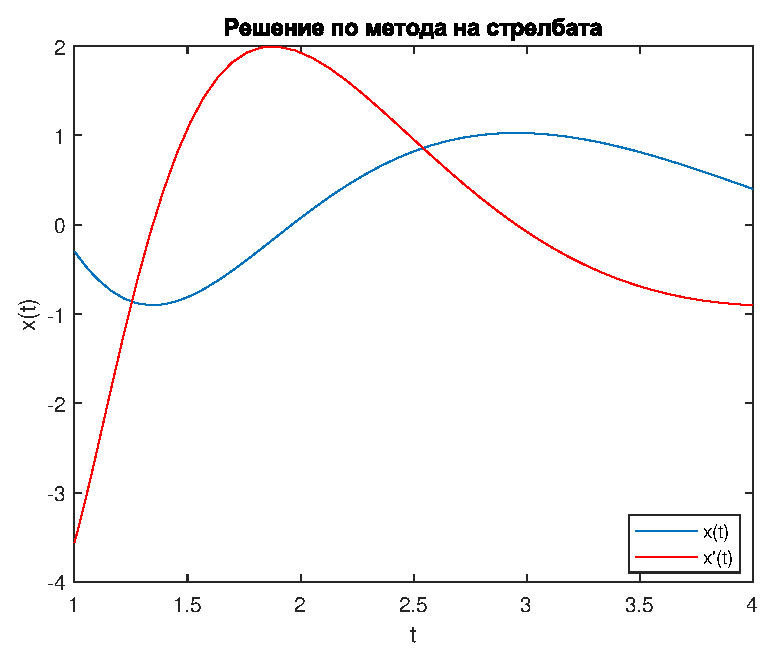
\includegraphics [width=4in]{fourthTask_01.eps}



\end{document}

